\chapter{The CF Pumping Lemma, Turing Machines}

\section{Non-context-free languages}

Based on \hyperref[theorem: CFG=PDA]{the equivalence of CFGs and PDAs}, there are some more corollaries we can see or easy to prove:

\begin{corollary}
    Every regular language is a CFL
\end{corollary}

\begin{corollary}
    If \(A\) is a CFL and \(B\) is regular then \(A \cap B\) is a CFL. 

    \begin{example}
        A: \(A = \{ a^nb^n | n \geq 0\} \) 
        B: \(B = \{ (ab)^* \} \) 
    \end{example}

    Proof sketch: while reading the input, the finite control of the PDA for \(A\) simulates the DFA for \(B\).  
\end{corollary}

Need to notice that the class of CFLs is not closed under \(\cap\) which is different from regular languages.

\begin{example}
    I will show an example where the intersection of 2 CFLs is not a CFL.

    \(L_1 = \{ a^n b^n c^m | n, m \geq 0 \} \) 

    \(L_2 = \{ a^m b^n c^n | n, m \geq 0 \} \) 

    \(L_1 \cap \L2 = \{ a^n b^n c^n | n \geq 0\} \) 

    Intuitively, to recognize the intersection of \(L_1\) and \(L_2\) we need to compare the count of \(a, b, c\). One stack can only handle the comparison of \(a\) and \(b\), but we have no extra stack for comparing \(c\).      
\end{example}

But the class of CFLs is closed under \(\cup, \circ, *\).  
\begin{note}
    Should try to prove its closed under union, concatenation and star!
\end{note}

\subsection{CF Pumping Lemma}
To prove a language is \textbf{not context free}, we need another tool:
\begin{example}\label{eg: 5.1}
    Let \(B = \{ 0^k 1^k 2^k | k \geq 0\} \), we will show that B is not a CFL. 
\end{example}

The tool we'll use is \textbf{Pumping Lemma for CFLs}: 
\begin{lemma}[Pumping Lemma for CFLs]
    If \(A\) is a CFL, then there is a number \(p\)(the pumping length) where, if \(s\) is any string in \(A\) of length at least \(p\), 
    then \(s\) may be divided into \textcolor{red}{five pieces \(s = uvxyz\)} satisfying the conditions
    \begin{enumerate}
        \item for each \(i \geq 0\), \(uv^i xy^iz \in A\)
        \item \(|vy| > 0\)
        \item \(|vxy| \leq p\)   
    \end{enumerate}    
\end{lemma}
\begin{proof}
    \begin{intuition}
    
    Proof IDEA: let \(s\) be a \textit{very long} string in \(A\), then the parsing tree for \(s\) must be very tall.  
    Then the parse tree must contain some long path from the start variable to the terminal symbol at a leaf. 
    On this long path, because of the pigeonhole principle, some variable \(R\) must repeat. 

    \begin{figure}[H]
        \centering
        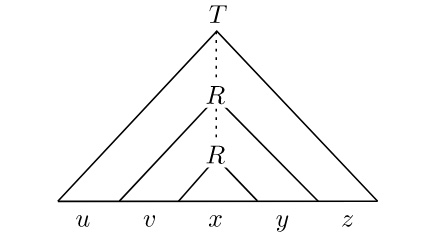
\includegraphics[width=0.6\textwidth]{f2.35-1.jpg}
        \caption{when \(s = uvxyz\) }
    \end{figure}

    This repetition allows us to replace the subtree under the second occurrence of \(R\) with the subtree under the first occurrence of \(R\) and still get a legal parse tree.  

    \begin{figure}[H]
        \centering
        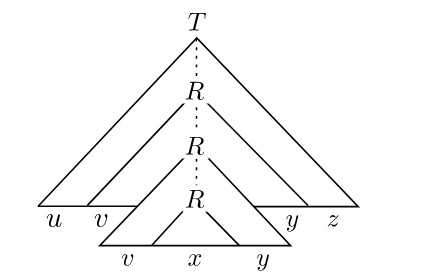
\includegraphics[width=0.6\textwidth]{f2.35-2.jpg}
        \caption{when \(s = uv^i xy^i z\) }
    \end{figure}

    Also \(v\) and \(y\) can repeat 0 time:

    \begin{figure}[H]
        \centering
        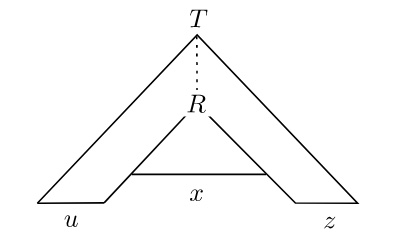
\includegraphics[width=0.6\textwidth]{f2.35-3.jpg}
        \caption{when \(s = uxz\) }
    \end{figure}
    \end{intuition}
\end{proof}

Let's go back to the \hyperref[eg: 5.1]{example}:
\begin{example}
    \(B = \{ 0^k1^k2^k | k \geq 0 \} \) 

    Proof by Contradiction:
    Assume that B \underline{is} a CFL.

    Based on CFL pumping lemma gives \(p\) as above, Let \(s = 0^p1^p2^p \in B\).  

    Pumping lemma says that can divide \(s = uwxyz\) satisfying the 3 conditions. 

    Condition 3 (\(|vxy| \leq p\)) implies that \(vxy\) can not contain both 0s and 2s. 

    So \(uv^2xy^2z\) has unequal numbers of 0s, 1s and 2s.
\end{example}

Another example:
\begin{example}
    Let \(F = \{ ww|w \in \Sigma^* \} \). \(\Sigma = \{ 0, 1 \} \). 
    
    Show: F is not a CFL.  

    Suppose \(F\) is a CFL, we try to construct a string which violate the CFL pumping lemma. 

    \begin{itemize}
        \item Try \(s_1 = 0^p10^p1\), we can choose \(x = 1\) of the middle, and v and y the left and right 0, and we can pump to this string. 
        \(\rightarrow\) \textcolor{red}{This is a bad choice to try to find a contradiction} 
        \item Try \(s_2 = 0^p 1^p 0^p 1^p\), now we can find the contradiction!
    \end{itemize}
\end{example}

\section{Turing Machines(TMs)}

\begin{example}
    
\end{example}

\begin{definition}[Turing Machine]
    
\end{definition}

TM recognizers and deciders:
